\documentclass[letterpaper]{article}
\usepackage[margin=1in]{geometry}
\usepackage[utf8]{inputenc}
\usepackage{textcomp}
\usepackage{amssymb}
\usepackage{natbib}
\usepackage{graphicx}
\usepackage{gensymb}
\usepackage{amsthm, amsmath, mathtools}
\usepackage[dvipsnames]{xcolor}
\usepackage{enumerate}
\usepackage{mdframed}
\usepackage[most]{tcolorbox}
\usepackage{csquotes}
% https://tex.stackexchange.com/questions/13506/how-to-continue-the-framed-text-box-on-multiple-pages

\tcbuselibrary{theorems}

\newcommand{\R}{\mathbb{R}}
\newcommand{\Z}{\mathbb{Z}}
\newcommand{\N}{\mathbb{N}}
\newcommand{\Q}{\mathbb{Q}}
\newcommand{\C}{\mathbb{C}}
\newcommand{\code}[1]{\texttt{#1}}
\newcommand{\mdiamond}{$\diamondsuit$}
\newcommand{\PowerSet}{\mathcal{P}}
\newcommand{\Mod}[1]{\ (\mathrm{mod}\ #1)}
\DeclareMathOperator{\lcm}{lcm}

%\newtheorem*{theorem}{Theorem}
%\newtheorem*{definition}{Definition}
%\newtheorem*{corollary}{Corollary}
%\newtheorem*{lemma}{Lemma}
\newtheorem*{proposition}{Proposition}


\newtcbtheorem[number within=section]{theorem}{Theorem}
{colback=green!5,colframe=green!35!black,fonttitle=\bfseries}{th}

\newtcbtheorem[number within=section]{definition}{Definition}
{colback=blue!5,colframe=blue!35!black,fonttitle=\bfseries}{def}

\newtcbtheorem[number within=section]{corollary}{Corollary}
{colback=yellow!5,colframe=yellow!35!black,fonttitle=\bfseries}{cor}

\newtcbtheorem[number within=section]{lemma}{Lemma}
{colback=red!5,colframe=red!35!black,fonttitle=\bfseries}{lem}

\newtcbtheorem[number within=section]{example}{Example}
{colback=white!5,colframe=white!35!black,fonttitle=\bfseries}{def}

\newtcbtheorem[number within=section]{note}{Important Note}{
        enhanced,
        sharp corners,
        attach boxed title to top left={
            xshift=-1mm,
            yshift=-5mm,
            yshifttext=-1mm
        },
        top=1.5em,
        colback=white,
        colframe=black,
        fonttitle=\bfseries,
        boxed title style={
            sharp corners,
            size=small,
            colback=red!75!black,
            colframe=red!75!black,
        } 
    }{impnote}
\usepackage[utf8]{inputenc}
\usepackage[english]{babel}
\usepackage{fancyhdr}
\usepackage{hyperref}
\usepackage{csquotes}
\usepackage{polynom}

\DeclareMathOperator{\ord}{ord}

\pagestyle{fancy}
\fancyhf{}
\rhead{Math 187A}
\chead{Friday, March 10, 2023}
\lhead{Lecture 18}
\rfoot{\thepage}

\setlength{\parindent}{0pt}

\begin{document}

\section{Modern Cryptography}
(Continued from previous notes.)

\subsection{Interlude: Elliptic Curves over the Reals}
\begin{definition}{Weierstrass Equation}{}
    A \textbf{Weierstrass equation} over the real numbers is an equation in $x$ and $y$ of the form 
    \[y^2 = x^3 + ax + b,\]
    where $a, b$ are fixed real numbers. The \textbf{discriminant} of the equation is 
    \[\Delta = -16(4a^3 + 27b^2)\]
    and the equation is singular when $\Delta = 0$. Otherwise, the equation is said to be nonsingular. 
\end{definition}

\begin{theorem}{}{}
    The Weierstrass equation $y^2 = x^3 + ax + b$ is nonsingular if and only if the cubic equation $x^3 + ax + b = 0$ has no repeated roots in the complex numbers.
\end{theorem}
Generally speaking, these (nonsingular) equations will look like one of the following:
\begin{center}
    \begin{tabular}{p{3in}|p{3in}}

        $y^2 = x^3 - x + 2$ & $y^2 = x^3 - x$ \\ 
        \hline 
        
        \bigskip 

        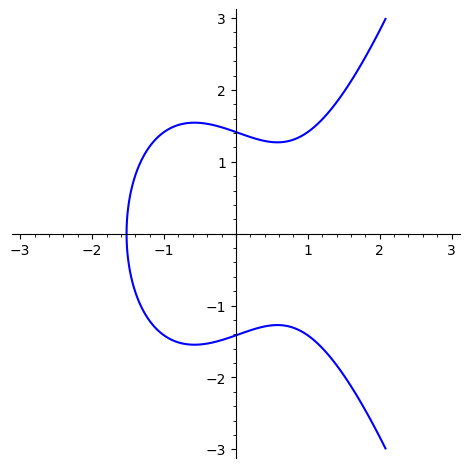
\includegraphics[scale=0.63]{../assets/weiers_1.png}
        &
        
        \bigskip 
        
        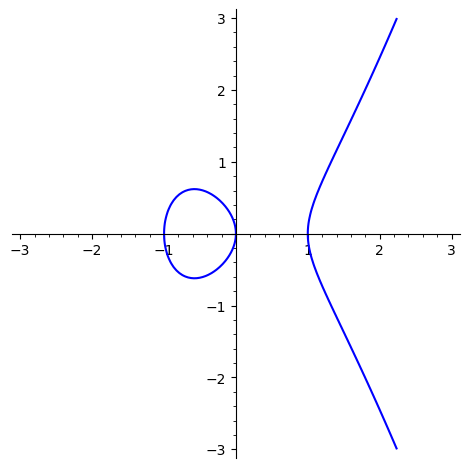
\includegraphics[scale=0.63]{../assets/weiers_2.png}
    \end{tabular}
\end{center}
These curves have a lot of important geometry. 
\begin{itemize}
    \item Observe that they are symmetric about the $x$-axis, i.e., they have vertical symmetry. Stated formally, if $(x, y)$ is a point satisfying $y^2 + x^3 + ax + b$, then its reflection $(x, -y)$ across the $x$-axis is also a point satisfying the same equation. If $P = (x, y)$ is a point on a curve defined by a Weierstrass equation, we define\footnote{We only invert the $y$-coordinate of $P$ to get $-P$, not both coordinates.} $-P$ to be this reflection $(x, -y)$.  
    \item If we pick any two points on the curve, the unique line that passes through those two points will (almost) have a unique ``other'' point of intersection with the curve.
\end{itemize}

\begin{mdframed}
    (Example.) Suppose we have the Weierstrass equation $y^2 = x^3 + 17$. This is nonsingular because \[\Delta = -16(4 \cdot 0^3 + 27 \cdot 17^2) = -16 \cdot 27 \cdot 17^2 \neq 0.\]
    Consider the points $P = (-2, 3)$ and $Q = (-1, 4)$. Both of these lie on the curve (see exercise \textbf{A}). THere is a unique ``secant'' line that passes through these two points; we can calculate its slope using the usual slope formula, 
    \[m = \frac{4 - 3}{(-1) - (-2)} = 1,\]
    and then we can find the equation of the secant line itself using point-slope form: 
    \[y - 4 = 1 \cdot (x - (-1)) \implies y = x + 5.\]
    How do we intersect this secant line with the curbe? Remember that this will consist of all $(x, y)$ points that satisfy both $y = x + 5$ and $y^2 = x^3 + 17$, so substituting the first equation into the second gives us 
    \begin{equation*}
        \begin{aligned}
            y^2 &= x^3 + 17 \\ 
                &\implies (x+5)^2 = x^3 + 17 \\ 
                &\implies x^2 + 10x + 25 = x^3 + 17 \\ 
                &\implies x^3 - x^2 - 10x - 8 = 0.
        \end{aligned}
    \end{equation*}
    We now need to solve this cubic equation. This generally isn't easy, but remember that we know $x = -2$ and $x = -1$ must be solutions to this equation, since $P = (-2, 3)$ and $Q = (-1, 4)$ are on the curve and on the line, and the $x$-coordinates of these points are precisely $-2$ and $-1$, respectively. Therefore, we know that 
    \[(x + 2)(x + 1) = x^2 + 3x + 2\]
    must divide $x^3 - x^2 - 10x - 8$. We can use polynomial long division to find the quotient (see exercise \textbf{B}). 

    \bigskip 

    We find that $x^3 - x^2 - 10x - 8 = (x + 2)(x + 1)(x - 4)$, so indeed the third solution to the cubic equation is $x = 4$ and thus plugging in $x = 4$ into the equation of line yields the point $R = (4, 9)$ (see exercise \textbf{C}). 
\end{mdframed}

\begin{mdframed}
    (Exercise \textbf{A}.) Check that $P = (-2, 3)$ and $Q = (-1, 4)$ are both on the curve defined by $y^2 = x^3 + 17$. 

    \begin{mdframed}
        For $P = (-2, 3)$, we have $3^2 = (-2)^3 + 17 \implies 9 = -8 + 17 = 9$; because both sides are equal, this point is on the curve. 

        \bigskip 

        For $Q = (-1, 4)$, we have $4^2 = (-1)^3 + 17 \implies 16 = -1 + 17 = 16$, so again this point is on the curve.
    \end{mdframed}
\end{mdframed}

\begin{mdframed}
    (Exercise \textbf{B}.) Use polynomial long division to divide $x^3 - x^2 - 10x - 8$ by $x^2 + 3x + 2$ and check that the quotient is $x - 4$ and the remainder is 0.

    \begin{mdframed}
        After performing long division, we find that the result is $x - 4$: 

        \smallskip 

        \polylongdiv[style=A]{x^3 - x^2 - 10x - 8}{x^2 + 3x + 2}
    \end{mdframed}
\end{mdframed}

\begin{mdframed}
    (Exercise \textbf{C}.) Check that $R = (4, 9)$ is on the curve defined by $y^2 = x^3 + 17$. 

    \begin{mdframed}
        \[y^2 = 9^2 = 81,\]
        \[x^3 + 17 = 4^3 + 17 = 64 + 17 = 81,\]
        and since both sides are equal, $R$ is on the curve.
    \end{mdframed}
\end{mdframed}

This is essentially what the example we've just gone over does: 
\begin{center}
    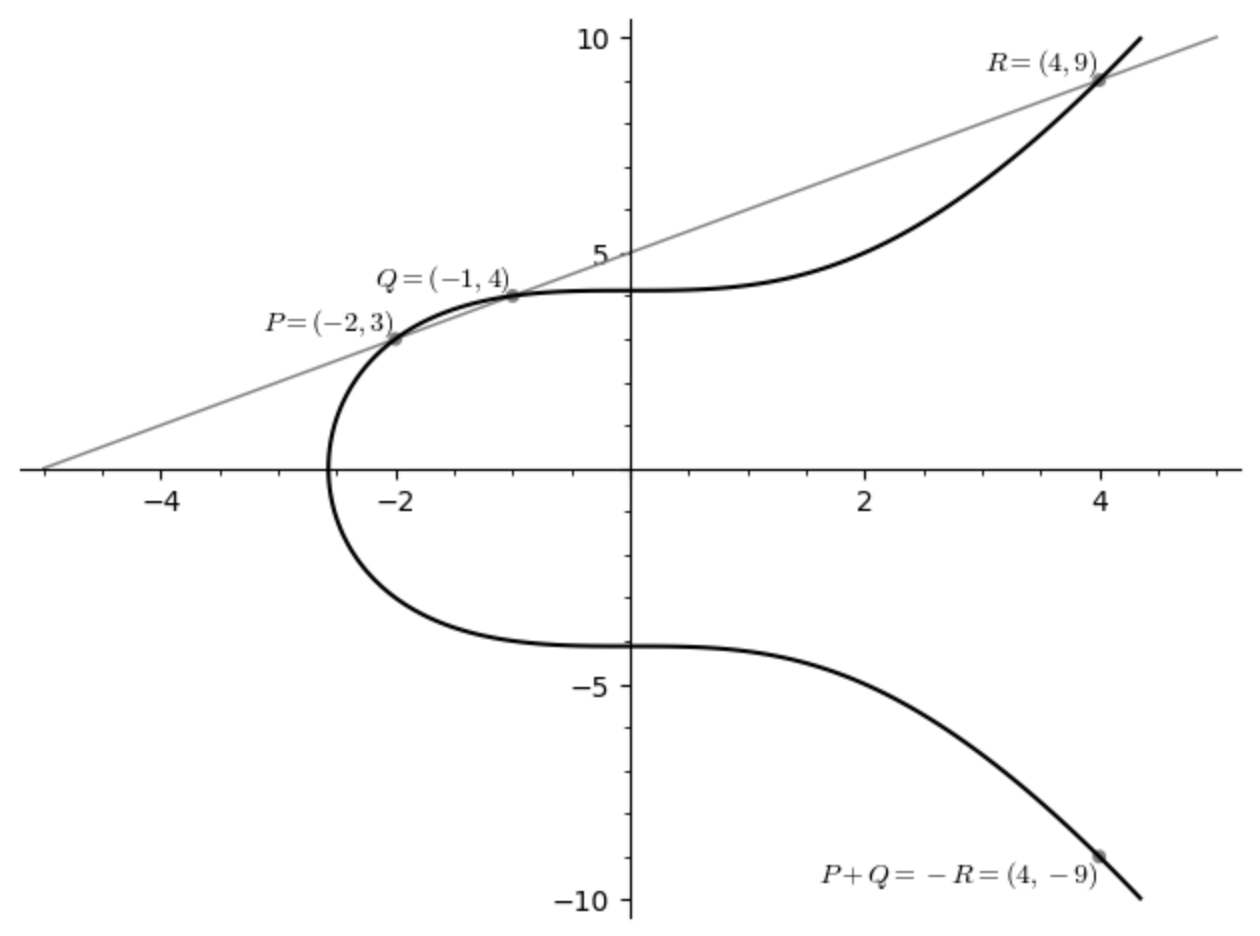
\includegraphics[scale=0.3]{../assets/weiers_3.png}

    \emph{Taken from Professor Agrawal's Notes.}
\end{center}

Notice here that we defined $P + Q = -R = (4, -9)$. In reality, however, this process may be more complicated than simply adding the $x$ and $y$ coordinates of the two points. 

\begin{mdframed}
    (Exercise.) 
    \begin{enumerate}[(a)]
        \item Let $S = (2, 5)$. Check that $S$ is on the same curve $y^2 = x^3 + 17$. 
        \begin{mdframed}
            \[y^2 = 25\]
            and 
            \[x^3 + 17 = 25,\]
            so $S$ is also on this curve. 
        \end{mdframed}
        \item What is the third point of the intersection on between the curve $y^2 = x^3 + 17$ and the second line connecting $Q = (-1, 4)$ and $S$?
        \begin{mdframed}
            Given the two points $Q$ and $S$, we can find their slopes: 
            \[m = \frac{4 - 5}{(-1) - 2} = \frac{-1}{-3} = \frac{1}{3}.\]
            Once we have the slope, we can find the equation of the line that passes through both points: 
            \[y - 4 = \frac{1}{3}(x - (-1)) \implies y - 4 = \frac{1}{3}(x + 1) \implies y = \frac{1}{3}x + \frac{1}{3} + 4 \implies y = \frac{1}{3}x + \frac{13}{3}.\]
            Remember that the intersection of the curve and the secant line will consist of all points $(x, y)$ such that both $y = \frac{1}{3}x + \frac{13}{3}$ and $y^2 = x^3 + 17$ are satisfied, so 
            \[y^2 = x^3 + 17 \implies \left(\frac{1}{3}x + \frac{13}{3}\right)^2 = x^3 + 17 \implies x^3 - \frac{1}{9}x^2 - \frac{26}{9}x + 17 - \frac{169}{9} = 0.\]
            Since this is a cubic function, there are three solutions. We know that $x = -1$ and $x = 2$ are solutions to this equation, so we can use long division to find the last solution. In particular, by dividing $x^3 - \frac{1}{9}x^2 - \frac{26}{9}x + 17 - \frac{169}{9}$ by $(x - 2)(x + 1) = x^2 - x - 2$,  
            
            \smallskip 

            \polylongdiv[style=A]{x^3 - \frac{1}{9}x^2 - \frac{26}{9}x + 17 - \frac{169}{9}}{x^2-x-2}

            \smallskip 

            we find that $x = -\frac{8}{9}$ is the last root. So, plugging this root into the equation of the line gives us \[\frac{1}{3}\left(-\frac{8}{9}\right) + \frac{13}{3} = \frac{109}{27},\] thus $R = \left(-\frac{8}{9}, \frac{109}{27}\right)$.
        \end{mdframed}
        \item What is $Q + S$? 
        \begin{mdframed}
            We have \[Q + S = -R = \left(-\frac{8}{9}, -\frac{109}{27}\right).\]
        \end{mdframed}
        \item With $P = (-2, 3)$ and $R = (4, 9)$ on $y^2 = x^3 + 17$ as above, what is $P + R$? 
        \begin{mdframed}
            The slope of $P$ and $R$ is 
            \[m = \frac{9 - 3}{4 - (-2)} = \frac{6}{6} = 1,\]
            so the equation of the line that passes through both points is \[y - 9 = 1(x - 4) \implies y = x - 4 + 9 \implies y = x + 5.\]
            Plugging this secant line equation into the Weierstrass equation gives us 
            \[y^2 = x^3 + 17 \implies (x + 5)^2 = x^3 + 17 \implies x^3 - x^2 - 10x - 8 = 0.\]
            Knowing that the two solutions to the intersection of the curve and the secant line are $x = -2$ and $x = 4$, we know that $(x + 2)(x - 4) = x^2 - 2x - 8$ must divide $x^3 - x^2 - 10x - 8$, so 
            
            \polylongdiv[style=A]{x^3 - x^2 - 10x - 8}{x^2 - 2x - 8}

            and so the last root must be $x = -1$. Plugging this $x = -1$ back into the secant line yields $y = 4$, so in particular $T = (-1, 4)$. Therefore, 
            \[P + R = -T = (-1, 4).\]
        \end{mdframed}
    \end{enumerate}
\end{mdframed}
Remember how we mentioned the (almost) unique ``other'' point? There are several caveats to consider. 
\begin{itemize}
    \item Suppose we choose $P = (-2, 3)$, the same point from the example. What does it mean to pick $P + P$ or $2P$? There's not\footnote{This is a problem particularly because the first step of this process involves finding such a secant line.} a unique secant line that passes through $P$ and $P$. However, recall in calculus that, if we think about the secant line through two points on a curve, and take the limit as one of the two points approaches the other, what we end up with is the tangent line. So, we can use this. In other words, we can define $P + P$ by going through the same process as usual, but using the tangent line of the curve at $P$. 
    
    \bigskip 

    Consider again $y^2 = x^3 + 17$. Using implicit differentiation, we have 
    \[2y\frac{dy}{dx} = 3x^2.\]
    Then, with $P = (x, y) = (-2, 3)$, plugging this in gives us 
    \[2 \cdot 3 \cdot \frac{dy}{dx}\bigg\rvert_{P} = 3(-2)^2 \implies \frac{dy}{dx}\bigg\rvert_{P} = 2.\]
    Finding the equation of the tangent line again using point-slope form like we did gives us 
    \[y - 3 = 2(x - (-2)) \implies y = 2x + 7.\]
    From there, the usual process follows. It should be noted that the $x$ in the point will be a double root of the cubic since the line is tangent to the curve \emph{at} $P$. 

    \begin{mdframed}
        (Exercise.) On the curve $y^2 = x^3 + 17$, define $2S$ where $S = (2, 5)$. Calculate $2S$. 

        \begin{mdframed}
            We have $2y\frac{dy}{dx} = 3x^2$, so with $S = (x, y) = (2, 5)$, we have 
            \[2(5)\frac{dy}{dx}\bigg\rvert_{S} = 3(2)^2 \implies \frac{dy}{dx}\bigg\rvert_{S} = \frac{3(2)^2}{2(5)} = \frac{12}{10} = \frac{6}{5}.\] From there, we can find the equation of the secant line,
            \[y - 5 = \frac{6}{5}(x - 2) \implies y = \frac{6}{5}(x - 2) + 5 \implies y = \frac{6}{5}x + \frac{13}{5}.\]
            Plugging this back into the Weierstrass equation yields 
            \[\left(\frac{6}{5}x + \frac{13}{5}\right)^2 = x^3 + 17 \implies \frac{36}{25}x^2 + \frac{156}{25}x + \frac{169}{25} = x^3 + 17 \implies x^3 - \frac{36}{25}x^2 - \frac{156}{25}x + \frac{256}{25} = 0.\] 
            We know that $x = 2$ is the only root, so we know that this must be a double root. Thus, we know that $(x - 2)(x - 2) = x^2 - 4x + 4$ must divide $x^3 - \frac{36}{25}x^2 - \frac{156}{25}x + \frac{256}{25}$. Therefore, 

            \polylongdiv[style=A]{x^3 - \frac{36}{25}x^2 - \frac{156}{25}x + \frac{256}{25}}{x^2 - 4x + 4}

            and thus $x = -\frac{64}{25}$ is the other root. Plugging this back into the secant line gives us $y = -\frac{59}{125}$, thus $T = \left(-\frac{64}{25}, -\frac{59}{125}\right)$ and $2S = -T = \left(-\frac{64}{25}, \frac{59}{125}\right)$.
        \end{mdframed}
    \end{mdframed}

    \item There is one situation when the line passing through two points(either the secant line through two distinct points or the tangent line at a single point) does not have a third point of intersection with the curve. This happens when the line ends up being vertical. We can deal with this \emph{by fiat}; that is, we declare that there is a point $O$ called the \emph{point at infinity}, which is a point on the curve defined by $y^2 = x^3 + 17$ and is also a point on every vertical line in the plane. It is its own negative. So, when we try to ``add'' two points and encounter the situation where a secant or tangent line is vertical, we declare the sum to be $O$.
    
    \begin{definition}{Elliptic Curve}{}
        Fix a nonsingular Weierstrass equation $y^2 = x^3 + ax + b$. The \textbf{elliptic curve} $E$ defined by this equation is the set of points $(x, y)$ satisfying this equation, together with a \emph{point of infinity} denoted $O$ and assumed by fiat to 
        \begin{itemize}
            \item lie on the curve, 
            \item lie on every vertical line in the plane, and 
            \item be its own reflection across the $x$-axis. 
        \end{itemize}
    \end{definition}

    \begin{theorem}{}{}
        Given any $P \in E$, where $E$ is an elliptic curve, we define $-P$ to be the reflection of $P$ across the $x$-axis. Given any two points $P, Q \in E$, there is a unique secant or tangent line passing through $P$ and $Q$, and this line has a unique third point of intersection with the curve; we define $P + Q$ to be the negative of this third point of intersection. Then, 
        \begin{itemize}
            \item Associativity: for any $P, Q, R \in E$, $(P + Q) + R = P + (Q + R)$.
            \item Commutativity: for any $P, Q \in E$, $P + Q = Q + P.$
            \item Identity: for any $P \in E$, $P + O = P.$
            \item Inverses: for any $P \in E$, $P + (-P) = O.$
        \end{itemize}
    \end{theorem}
    \textbf{Remark:} The above is saying that $E$ is an ``abelian'' group\footnote{If you've taken group theory, this should be familiar. Don't worry if you aren't familiar with this.}.
\end{itemize} 

\begin{theorem}{Elliptic Curve Addition Formula}{3-10:1}
    Suppose $P = (x_1, y_1)$ and $Q = (x_2, y_2)$ are both points on the curve $y^2 = x^3 + ax + b$. Then, define 
    \[\lambda = \begin{cases}
        \frac{y_2 - y_1}{x_2 - x_1} & \text{if } P \neq Q \\ 
        \frac{3x_1^2 + a}{2y_1} & \text{if } P = Q 
    \end{cases}.\]
    If $\lambda$ is defined (i.e., the denominator above is nonzero), then set 
    \[\nu = y_1 - \lambda x_1\]
    \[x_3 = \lambda^2 - x_1 - x_2\]
    \[y_3 = \lambda x_3 + \nu.\]
    Then, $P + Q = (x_3, -y_3)$. 
\end{theorem}

\begin{mdframed}
    (Exercise.) Consider the Weierstrass equation $y^2 = x^3 - 2x$. 

    \begin{enumerate}[(a)]
        \item Verify that this equation is nonsingular. Let $E$ be the corresponding elliptic curve. 
        \begin{mdframed}
            Computing the discriminant with $a = -2$ and $b = 0$ gives us
            \[\Delta = -16(4(-2)^3 + 27(0)^2) = -16 \cdot 4(-2)^3 \neq 0,\]
            so this equation is nonsingular. 
        \end{mdframed}
        \item Verify that $P = (0, 0)$ is on the curve. What is $2P$? 
        \begin{mdframed}
            The left-hand side has $0^2 = 0$ and the right-hand side has $0^3 - 2(0) = 0$, so it follows that $P$ is on the curve. 

            \bigskip 

            TODO 
        \end{mdframed}
        \item Verify that $Q = (-1, 1)$ is on the curve. What is $2Q$?
        \begin{mdframed}
            TODO 
        \end{mdframed}
        \item What is $P + Q$? 
        \begin{mdframed}
            TODO 
        \end{mdframed}
        \item What is $3Q$? 
        \begin{mdframed}
            TODO 
        \end{mdframed}
        \item What is $4Q$? 
        \begin{mdframed}
            TODO 
        \end{mdframed}
        \item What is $5Q$? 
        \begin{mdframed}
            TODO 
        \end{mdframed}
    \end{enumerate}
\end{mdframed}

\begin{definition}{Order}{}
    Suppose $P$ is a point on an elliptic curve $E$. The order of $P$, denoted $\ord_{E}(P)$, is the smallest positive integer $n$ such that $nP = O$, if such an integer exists. Otherwise, the order of $P$ is $\infty$. 
\end{definition}

\begin{mdframed}
    (Exercise.) Let $E$ be the elliptic curve defined by the Weierstrass equation $y^2 = x^3 - 4x$. Find the order of the following points. 
    \begin{enumerate}[(a)]
        \item $P = (-2, 0)$
        \begin{mdframed}
            TODO 
        \end{mdframed}
        \item $Q = (0, 0)$
        \begin{mdframed}
            TODO 
        \end{mdframed}
        \item $P + Q$
        \begin{mdframed}
            TODO 
        \end{mdframed}
    \end{enumerate}
\end{mdframed}


\subsection{Interlude: Elliptic Curves Mod a Prime}
We now fix a prime $p$. For technical reasons that are not worth lingering on for our purposes here, we assume\footnote{In applications to cryptography, $p$ will be very large anyways.} that $p \geq 5$. 

\begin{definition}{Integral Weierstrass Equation}{}
    A Weierstrass equation $y^2 = x^3 + ax + b$ is \textbf{integral} if $a$ and $b$ are integers. We then say that the equation is singular mod $p$ if $\Delta \equiv 0 \Mod{p}$. Otherwise, it is nonsingular mod $p$. 
\end{definition}

\begin{mdframed}
    (Example.) Suppose we have the Weierstrass equation $y^2 = x^3 + 17$. It is integral since $a = 0$ and $b = 17$ are integers. Then, we calculated earlier that \[\Delta = -16 \cdot 27 \cdot 17^2.\] The only primes this is divisible by are 2, 3, and 17. Thus, the equation $y^2 = x^3 + 17$ is singular mod $p = 17$, but nonsingular otherwise (recall that we are ruling out $p = 2, 3$).
\end{mdframed}

\begin{mdframed}
    For each of the following integral Weierstrass equations, find all primes $p \geq 5$ such that the equation is singular mod $p$. 
    \begin{enumerate}
        \item $y^2 = x^3 - 2x$    
        \begin{mdframed}
            TODO 
        \end{mdframed}
        \item $y^2 = x^3 + x + 1$
        \begin{mdframed}
            TODO 
        \end{mdframed}
        \item $y^2 + x^3 - 1$
        \begin{mdframed}
            TODO 
        \end{mdframed}
    \end{enumerate}
\end{mdframed}
So, when we have an integral Weierstrass equation $y^2 = x^3 + ax + b$, we can consider its ``solutions mod $p$.'' By this, we mean integers $(x, y)$ such that $y^2 \equiv x^3 + ax + b \Mod{p}$. 

\begin{mdframed}
    (Example.) Suppose $p = 7$ and consider the Weierstrass equation $y^2 = x^3 + 17$. Then, $(1, 2)$ is a solution to the equation mod $p$ because 
    \[y^2 = 2^2 = 4 \equiv 18 = 1^3 + 17 = x^3 + 17 \Mod{7}.\]
\end{mdframed}
Let's define that, if $x, y, x', y'$ are all integers, then 
\[(x, y) \equiv (x', y') \Mod{p}\]
means that $x \equiv x' \Mod{p}$ and $y \equiv y' \Mod{p}$. Notice that, if $(x, y)$ is a solution mod $p$ of $y^2 = x^3 + ax + b$, then so is any pair of integers that is congruent mod $p$. 
\begin{mdframed}
    (Example.) In the above example, $(1, 9), (8, 2), (-6, 9)$ are all congruent mod 7 to $(1, 2)$, and they are all also solutions mod 7 to $y^2 = x^3 + 17$. 
\end{mdframed}    
We'll typically consider only solutions $(x, y)$ where $0 \leq x, y < p$ in order to avoid having to list off all the congruent solutions.

\begin{theorem}{}{}
    Suppose $y^2 = x^3 + ax + b$ is an integral Weierstrass equation which is nonsingular mod $p$. The corresponding elliptic curve mod $p$ is the set $E$ of solutions mod $p$ to the equation, together with an extra point at infinity called $O$. 

    \bigskip 

    Suppose $P \in E$. We define $-P$ as follows: 
    \begin{itemize}
        \item If $P = O$, then $-P = O$ as well.
        \item If $P = (x, y)$, then $-P = (x, -y \Mod{p})$. 
    \end{itemize}
    Then, $-P$ is in fact an element of $E$. 

    \bigskip 

    Moreover, suppose $P, Q \in E$. We define $P + Q$ as follows: 
    \begin{itemize}
        \item If $P = O$, then $P + Q = Q$. 
        \item If $Q = O$, then $P + Q = P$. 
        \item If $P = (x_1, y_1)$ and $Q = (x_2, y_2)$ are both solutions mod $p$ of $y^2 = x^3 + ax + b$, then 
        \begin{itemize}
            \item If $P \neq Q$ and $x_2 - x_1$ is not invertible mod $p$, set \[P + Q = O.\]
            \item If $P = Q$ and $y_1$ is not invertible mod $p$, set $P + Q = 2P = O$. 
            \item Otherwise, define\footnote{You compute the inverse mod $p$ first, and then multiply that and mod that by $p$.}
            \[\lambda = \begin{cases}
                (y_2 - y_1)(x_2 - x_1)^{-1} \Mod{p} & \text{if } P \neq Q \\ 
                (3x_1^2 + a)(2y_1)^{-1} \Mod{p} & \text{if } P = Q 
            \end{cases}.\]
            Then, set 
            \[\nu = y_1 - \lambda x_1 \Mod{p}\]
            \[x_3 = \lambda^2 - x_1 - x_2 \Mod{p}\]
            \[y_3 = \lambda x_3 + \nu \Mod{p}\]
            Then, $R = (x_3, y_3)$ is a solution mod $p$ and we define $P + Q = -R = (x_3, -y_3 \Mod{p})$. 
        \end{itemize}
    \end{itemize}
    Then, 
    \begin{itemize}
        \item Associativity: for any $P, Q, R \in E$, $(P + Q) + R = P + (Q + R)$.
        \item Commutativity: for any $P, Q \in E$, $P + Q = Q + P.$
        \item Identity: for any $P \in E$, $P + O = P.$
        \item Inverses: for any $P \in E$, $P + (-P) = O.$
    \end{itemize}
\end{theorem}

\begin{mdframed}
    (Example.) Consider $p = 7$ and $y^2 = x^3 + 17 \equiv x^3 + 3 \Mod{7}$. We already saw that $P = (1, 2)$ is a solution to this equation. We also know that $Q = (3, 4)$ is also a solution to this equation. With this in mind, how do we compute $P + Q$ in ``two'' different ways?
    \begin{itemize}
        \item Using the above formula carefully, notice that $P \neq Q$ and $x_2 - x_1 = 3 - 1 = 2$ is invertible mod 7 because $\gcd(2, 7) = 1$. Its inverse\footnote{Generally, you would want to use the extended Euclidian algorithm.} is 4. Thus, 
        \[\lambda = (y_2 - y_1)(x_2 - x_1)^{-1} \Mod{p} = (4 - 2)(3 - 1)^{-1} \Mod{7} = 2 \cdot 4 \Mod{7} = 1.\]
        From there, 
        \[\nu = y_1 - \lambda x_1 \Mod{p} = 1\]
        \[x_3 = \lambda^2 - x_1 - x_2 \Mod{p} = 4\]
        \[y_3 = \lambda x_3 + \nu \Mod{p} = 5.\]
        Therefore, $R = (4, 5)$ and $P + Q = -R = (4, -5 \Mod{7}) = (4, 2)$. 

        \item The other way is to remember the geometry that underlies these formulas and use the geometry to guide your calculations. Just remember that you're trying to do everything mod 7. So, begin by computing the slope of the two points using rise-over-run, but since we need to do this calculation mod 7, isntead of dividing, we multiply by a modular inverse. In other words, we compute 
        \[m = (4 - 2)(3 - 1)^{-1} = 2 \cdot 2^{-1} \equiv 2 \cdot 4 = 8 \equiv 1 \Mod{7}.\]
        This is the same value we found with $\lambda$ above. Now, the next step is to use the point-slope form to find the equation of the secant line; we know that it has slope 1, and it passes through the point $(1, 2)$, so its equation should be \[y - 2 = 1(x - 1) \implies y = x + 1.\]
        The $y$-intercept here matches what we computed for $\nu$ above. We now want to intersect this secant line with the curve. So, we substitute $y = x + 1$ into $y^2 = x^3 + 3$ and get \[x^3 - x^2 - 2x + 2 = 0.\]
        We now need to find the roots of this cubic mod 7. We know that 1 and 3 are roots, so $(x - 1)(x - 3) = x^2 - 4x + 3$ must divide this cubic. Performing polynomial long division ``mod 7'' gives us $x - 4$ as the result, so the third point of intersection of the secant line must have $x = 4$, so $y = 5$. This gives us $R = (4, 5)$. Therefore, 
        \[P + Q = (1, 2) + (3, 4) = (4, -5 \Mod{7}) = (4, 2).\]
    \end{itemize}
\end{mdframed}

\begin{definition}{Order}{}
    Suppose $P$ is a point on an elliptic curve $E$ mod $p$. The \textbf{order} of $P$, denoted $\ord_{E}(P)$, is the smallest positive integer $n$ such that $nP = O$. 
\end{definition}
Unlike in the real case, we don't need to worru about the infinite order anymore. 

\bigskip 

We also have the analogs of the First and Second Lemmas about Orders. 
\begin{lemma}{First Lemma About Orders for Elliptic Curves}{}
    Let $E$ be an elliptic curve mod $p$ and suppose $P \in E$. If $mP = O$, then $\ord_{E}(P)$ divides $m$. 
\end{lemma}

\begin{lemma}{Second Lemma About Orders for Elliptic Curves}{}
    Let $E$ be an elliptic curve mod $p$ and suppose $P \in E$. Let $k = \ord_{E}(P)$. Then, \[iP \equiv jP \Mod{p}\] if and only if $i \equiv j \Mod{k}$. In particular, the points $O, P, 2P, 3P, \hdots, (k - 1)P$ are all incongruent mod $p$.
\end{lemma}
Having developed this theory, we can now state the basic problem that underlies elliptic curve cryptography. 
\begin{mdframed}
    (Elliptic Curve Discrete Logarithm Problem.) Suppose that you're given a prime $p$, an elliptic curve $E \Mod{p}$, and a point $P \in E$. Further suppose that $Q \in E$ is known to be a multiple of $P$. Find the discrete logarithm base $P$ of $Q$, i.e., the unique integer $k$ such that $0 \leq k < \ord_{E}(P)$ such that $Q = mP$. 
\end{mdframed}
The naive method for doing this is to just try all values of $k$ starting from $k = 0$ to $k = \ord_{E}(P) - 1$, but if $\ord_{E}(P)$ is very large, then this will be very slow. There are no methods that can help us find $k$ substantially faster in general, so we can choose $p, E, P$ in a way that makes the Elliptic Curve Discrete Logarithm Problem intractable for an adversary. 

\end{document}